\header{
    \headtitle{Le soldat belge} \label{le-soldat-belge}
    %
    \insertComment{Chanson populaire et patriotique belge, créée dans les années 1920.}{}
}

\enluminure{4}{\href{https://www.youtube.com/watch?v=hdDpqLnMLww}{C}}{'était} un soir sur les bords de l’Yser,
\\Un soldat belge qui montait la faction.
\\Vinrent à passer trois gardes militaires,
\\Parmi lesquels était le Roy Albert.
\\Qui vive là ? lui crie la sentinelle,
\\Qui vive là ? Vous ne passerez pas !
\\Si vous passez craignez ma baïonnette,
\\Retirez-vous, vous ne passerez pas ! \bissimple
\\Halte-là !
\\\\Le Roy Albert en fouillant dans ses poches,
\\Tiens, lui dit-il, et laisse-moi passer.
\\Non, répondit la brave sentinelle,
\\L’argent n’est rien pour un vrai soldat belge.
\\Dans mon pays, je cultivais la terre,
\\Dans mon pays, je gardais les brebis,
\\Mais, maintenant que je suis militaire,
\\Retirez-vous, vous ne passerez pas ! \bissimple
\\Halte-là !
\\\\Le Roy Albert dit à ses camarades :
\\Fusillons-le, c’est un mauvais sujet.
\\Fusillons-le à la lueur des astres,
\\Fusillons-le, c’est un mauvais sujet.
\\Fusillez-moi, lui dit la sentinelle,
\\Fusillez-moi, vous ne passerez pas.
\\Si vous passez, craignez ma baïonnette.
\\Retirez-vous, vous ne passerez pas ! \bissimple
\\Halte-là !

\breakpage
Le lendemain, au grand conseil de guerre,
\\Le Roy Albert lui demanda son nom.
\\Tiens, lui dit-il, voilà la croix de guerre,
\\La croix de guerre et la décoration.
\\Que va-t-elle dire, ma bonne et tendre mère,
\\Que va-t-elle dire en me voyant si beau ?
\\La croix de guerre est à ma boutonnière
\\Pour avoir dit : vous ne passerez pas ! \bissimple
\\Halte-là !
\bigskip
\bigskip
\begin{center}
\centering
    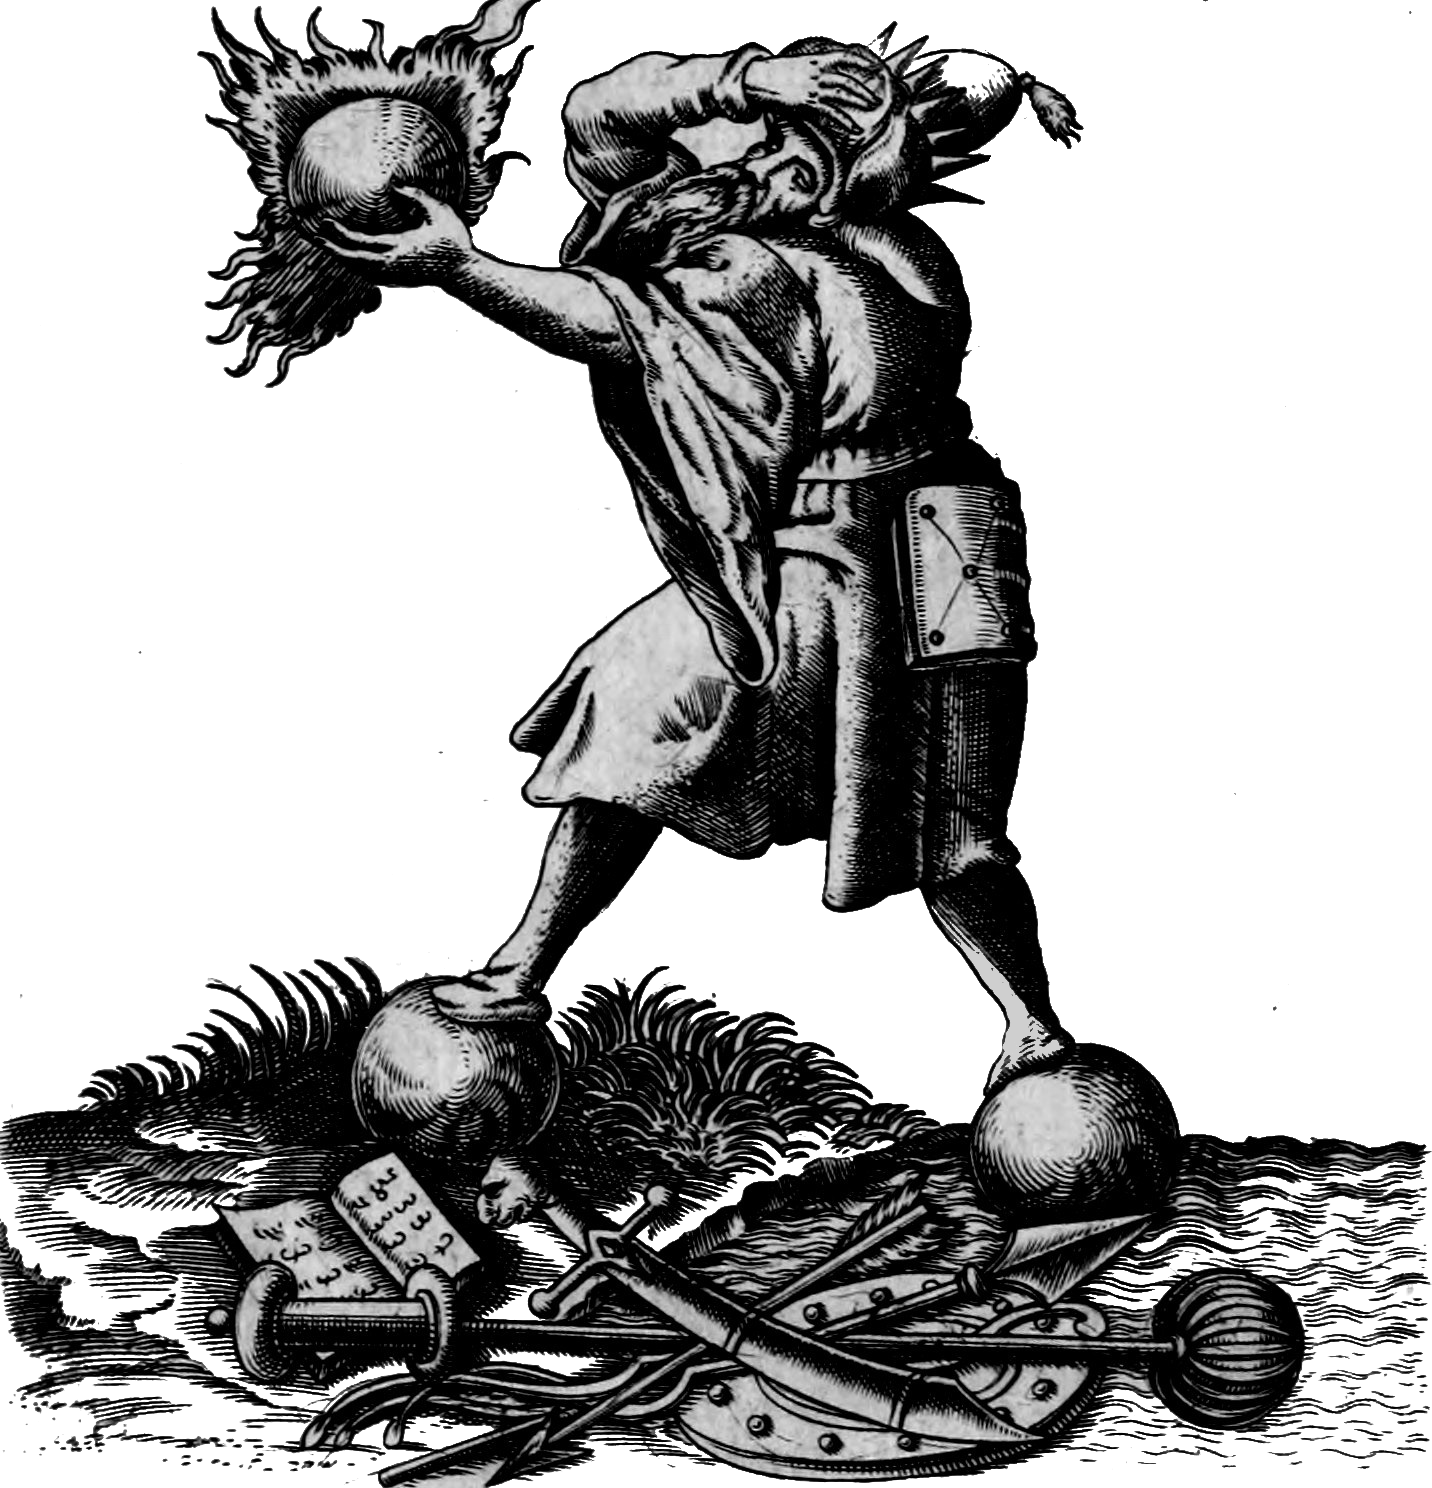
\includegraphics[width=1\textwidth]{images/brev57.png}
 \end{center}

\breakpage